\chapter[Criação e Uso de Conectores]{Criação e Uso de Conectores}

Neste capítulo veremos como criar um conector, gerenciá-lo e utilizá-lo através da criação de um serviço de proxy customizado.

\section{Criação de conectores}

(REFERENCIAR https://docs.wso2.com/display/ESB480/Working+with+Connectors)
A criação de conectores é feita para encapsular a API de um serviço externo, disponibilizando operações que podem ser acessadas por aplicações de forma simplificada. Os conectores são definidos por templates, que contém todas as operações disponíveis bem como propriedades (ou valores) necessárias para a execução da operação do serviço solicitada.

A ferramenta WSO2 ESB possui diversos conectores que permitem o uso de serviços tais como Twitter, Facebook, eBay, Foursquare, Github e Gmail. Também  é possível criar conectores customizados e utilizá-los no WSO2 ESB.

Para a criação do conector deste manual, foi utilizada a aplicação EnTurma, desenvolvida por alunos da Universidade de Brasília para o projeto final das disciplinas Gerenciamento de Projetos e Portifólios e Métodos de Desenvolvimento de Software durante o primeiro semestre do ano letivo de 2015. A aplicação pode ser acessada através do link \url{http://www.projetoenturma.com.br/}. O objetivo é exibir de forma mais intuitiva dados referentes à educação básica brasileira. A aplicação possui três funcionalidades:
\begin{itemize}
\item Visualização de Ranking: de acordo com o ano e turma escolhidos, é exibida uma lista ordenada de acordo com índices de evasão, rendimento escolar, distorção de idade com relação à recomendada para a turma escolhida e dados da prova IDEB (se foi aplicada no ano escolhido).
\item Relatórios de turmas: são exibidos os mesmos dados para a visualização do ranking, mas apenas apra uma truma escolhida de determinada localidade. É possível determinar a partir de qual ano os dados devem ser exibidos, mostrando a evolução dos dados.
\item Comparar turmas: dadas duas turmas, é feita uma comparação. Assim é possível verificar se existem turmas com melhores desempenhos e proporcionar a pesquisa de melhores metodologias de ensino e promover a melhroria da educação brasileira.
\end{itemize}

Neste manual será criado um conector customizado para esta aplicação. Também serão exibidos como gerenciá-lo no ESB e o uso deste conector em uma segunda aplicação.

\subsection{Estrutura do conector}

Para a criação do conector é necessário o acesso à API do serviço para o qual este será criado. A estrutura do conector varia de acordo com o tipo de API utilizada: REST APIs permitem a criação de conectores apenas com arquivos de configuração em formato XML, enquanto JAVA APIs necessitam que os arquivos de configuração sejam escritos em formato XML e utilizam (ou indicam) as operações escritas em Java.

A aplicação para o qual será criado o conector disponibiliza o acesso de seus serviços via REST API. Assim sendo, a estrutura do conector será:

\begin{figure}[htb]
\centering
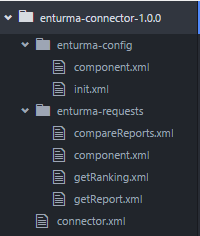
\includegraphics[width=0.5\textwidth]{figuras/estrutura_conector.PNG}
\caption{Estrutura do conector.}
\label{estrutura_conector}
\end{figure}

\begin{itemize}
\item As pastas devem conter os conjuntos de templates de operações oferecidas pelo serviço. A criação de várias pastas é recomendada para o agrupamento de operações do mesmo tipo.
\item Cada pasta é considerada um componente do conector. O arquivo \textit{component.xml} contém a declaração e descrição das operações disponíveis.
\item Cada operação deve ser descrita em um arquivo .xml. As operações serão identificadas no arquivo \textit{component.xml}, onde serão denominadas e associadas ao arquivo que as descrevem.
\item É recomendado que as configurações (parâmetros) essenciais para o uso do serviço estejam descritas em uma pasta \textit{<nome\_conector>-config}.
\item O arquivo \textit{connector.xml} contém a descrição de todos os componentes do conector.
\end{itemize}

\subsubsection{Template para acesso à operações do serviço}
As operações disponibilizadas para uso do serviço são descritas através de templates. Quando a operação é chamada por uma aplicação, os parâmetros solicitados são substituídos pelos valores fornecidos e a operação é executada de acordo com a descrição do template.

Veja na figura abaixo o template da operação que permite a recuperação de dados sobre o ranking de dado ano e grade (parâmetros usados pelo template).

\begin{figure}[htb]
\centering
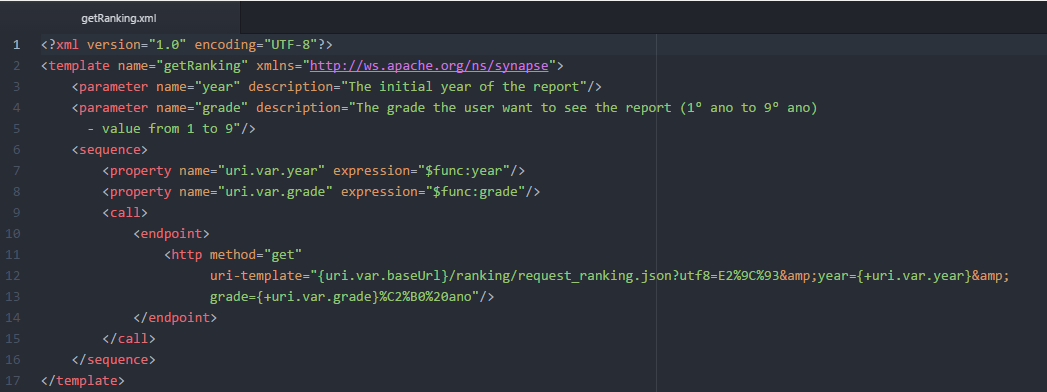
\includegraphics[width=1.0\textwidth]{figuras/operacao_ranking.PNG}
\caption{Template da operação \textit{getRanking}.}
\label{operacao_ranking}
\end{figure}

A operação \textit{getRanking} é uma chamada do método GET da API REST no link especificado pelo \textit{uri-template}. O retorno desta operação é o resultado desta chamada.

A URL base da aplicação é inicializada na operação \textit{init} do serviço.
\begin{figure}[htb]
\centering
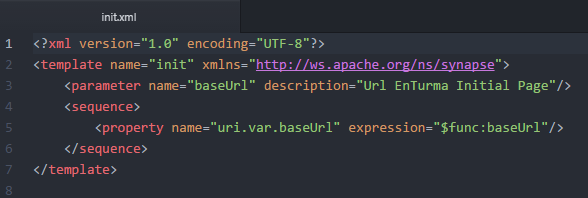
\includegraphics[width=1.0\textwidth]{figuras/operacao_init.PNG}
\caption{Template da operação \textit{init}.}
\label{operacao_init}
\end{figure}

\subsubsection{Descrição do componente do conector}
Uma vez que as operações estão definidas, o componente pode ser descrito. Para cada pasta - conjunto de operações - deve ser criado um arquivo onde o componente será descrito. O conector criado para este manual possui dois componentes: "enturma-config" e "enturma-requests". Ambos possuem um arquivo chamado \textit{component.xml}, onde as operações de tal componente são descritas. Na figura abaixo pode-se ver a descrição do componente "enturma-requests".

\begin{figure}[htb]
\centering
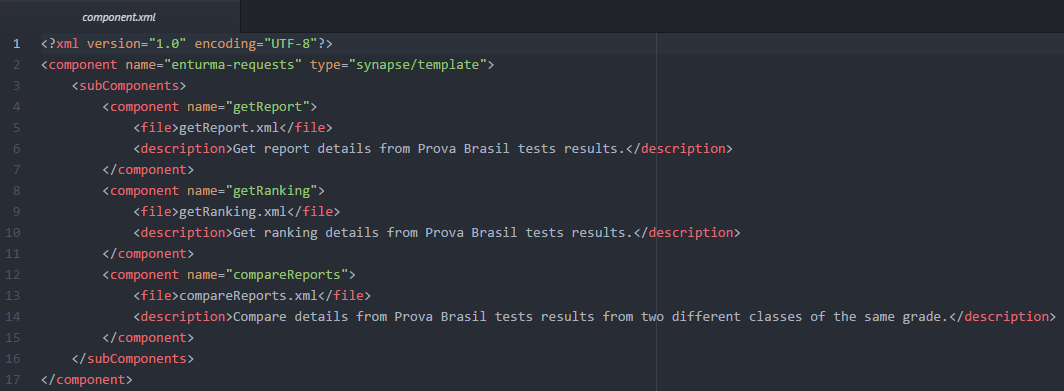
\includegraphics[width=1.0\textwidth]{figuras/componente.PNG}
\caption{Descrição do componente "enturma-requests".}
\label{componente}
\end{figure}


\subsubsection{Descrição do conector}
A definição do nome no ESB, o pacote e os componentes do conector são descritos no arquivo \textit{connector.xml}. A descrição dos componentes são recomendadas.

\begin{figure}[htb]
\centering
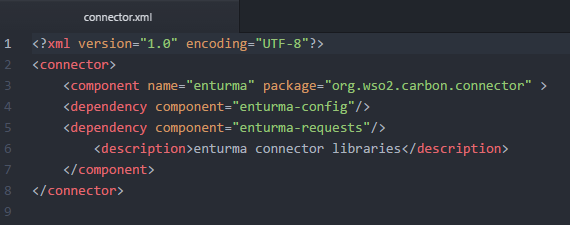
\includegraphics[width=1.0\textwidth]{figuras/connectorxml.PNG}
\caption{Descrição do conector "enturma".}
\label{connectorxml}
\end{figure}


Para finalizar, o conector deve ser compactado em uma pasta .zip (apenas neste formato). O arquivo criado neste manual foi denominado \textit{enturma-connector-1.0.0.zip}.

\section{Adição do conector ao ESB}
No ESB será adicionado o arquivo \textit{enturma-connector-1.0.0.zip}. Para isto, acesse o menu indicado na figura abaixo, escolha o arquivo .zip criado e faça o \textit{upload} deste.

\begin{figure}[htb]
\centering
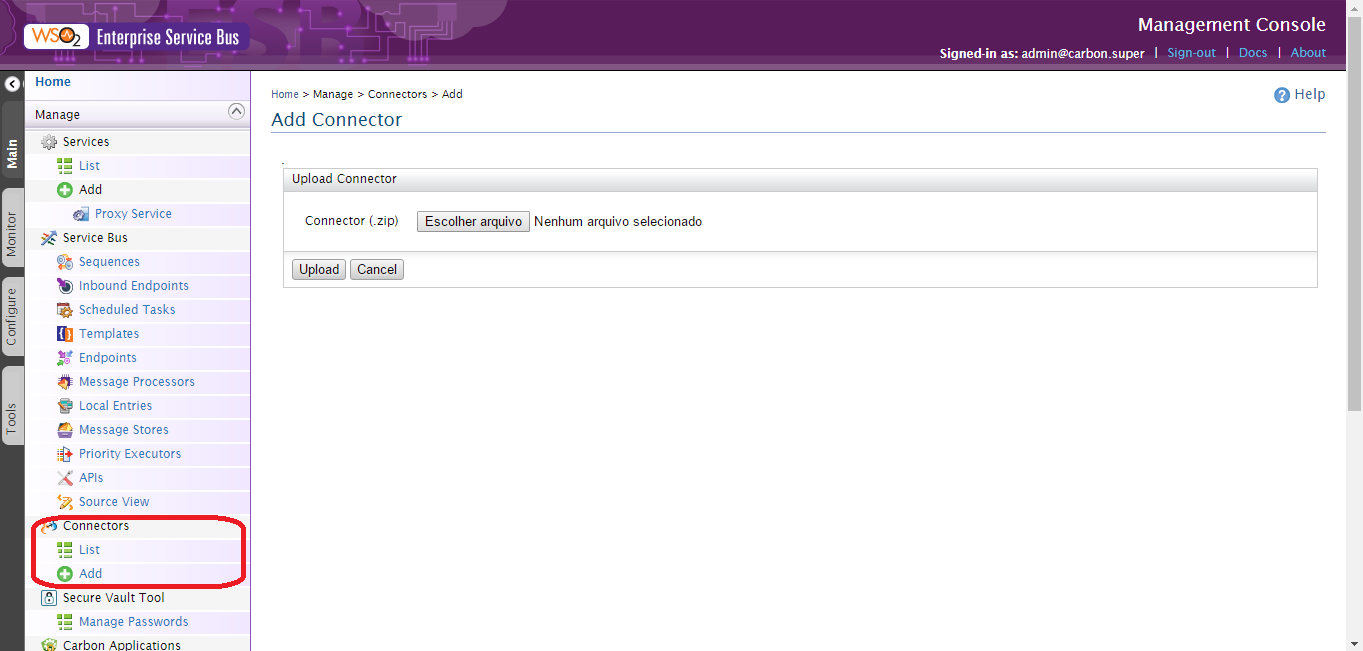
\includegraphics[width=1.0\textwidth]{figuras/add_connector.PNG}
\caption{Adição do conector "enturma" ao ESB.}
\label{add_connector}
\end{figure}

Ao realizar o \textit{upload} do arquivo, as operações do serviço descritos no conector poderão ser acessadas se incluídas em um serviço disponibilizado no ESB. A criação do serviço customizado para acessar as operações do conector "enturma" será descrita logo adiante neste manual.

A lista de conectores deverá ser atualizada. Para que possa ser utilizado, o conector deverá ser ativado: apenas clique no \textit{status} correspondente ao conector. As operações disponíveis para uso através do conector podem ser vistos ao clicar no conector identificado pelo nome descrito no arquivo \textit{connector.xml}.

\section{Criação do serviço no ESB}


\section{Uso do serviço ESB em uma aplicação}


